\documentclass[runningheads,11pt]{llncs}\usepackage[]{graphicx}\usepackage[]{color}
%% maxwidth is the original width if it is less than linewidth
%% otherwise use linewidth (to make sure the graphics do not exceed the margin)
\makeatletter
\def\maxwidth{ %
  \ifdim\Gin@nat@width>\linewidth
    \linewidth
  \else
    \Gin@nat@width
  \fi
}
\makeatother

\definecolor{fgcolor}{rgb}{0.345, 0.345, 0.345}
\newcommand{\hlnum}[1]{\textcolor[rgb]{0.686,0.059,0.569}{#1}}%
\newcommand{\hlstr}[1]{\textcolor[rgb]{0.192,0.494,0.8}{#1}}%
\newcommand{\hlcom}[1]{\textcolor[rgb]{0.678,0.584,0.686}{\textit{#1}}}%
\newcommand{\hlopt}[1]{\textcolor[rgb]{0,0,0}{#1}}%
\newcommand{\hlstd}[1]{\textcolor[rgb]{0.345,0.345,0.345}{#1}}%
\newcommand{\hlkwa}[1]{\textcolor[rgb]{0.161,0.373,0.58}{\textbf{#1}}}%
\newcommand{\hlkwb}[1]{\textcolor[rgb]{0.69,0.353,0.396}{#1}}%
\newcommand{\hlkwc}[1]{\textcolor[rgb]{0.333,0.667,0.333}{#1}}%
\newcommand{\hlkwd}[1]{\textcolor[rgb]{0.737,0.353,0.396}{\textbf{#1}}}%
\let\hlipl\hlkwb

\usepackage{framed}
\makeatletter
\newenvironment{kframe}{%
 \def\at@end@of@kframe{}%
 \ifinner\ifhmode%
  \def\at@end@of@kframe{\end{minipage}}%
  \begin{minipage}{\columnwidth}%
 \fi\fi%
 \def\FrameCommand##1{\hskip\@totalleftmargin \hskip-\fboxsep
 \colorbox{shadecolor}{##1}\hskip-\fboxsep
     % There is no \\@totalrightmargin, so:
     \hskip-\linewidth \hskip-\@totalleftmargin \hskip\columnwidth}%
 \MakeFramed {\advance\hsize-\width
   \@totalleftmargin\z@ \linewidth\hsize
   \@setminipage}}%
 {\par\unskip\endMakeFramed%
 \at@end@of@kframe}
\makeatother

\definecolor{shadecolor}{rgb}{.97, .97, .97}
\definecolor{messagecolor}{rgb}{0, 0, 0}
\definecolor{warningcolor}{rgb}{1, 0, 1}
\definecolor{errorcolor}{rgb}{1, 0, 0}
\newenvironment{knitrout}{}{} % an empty environment to be redefined in TeX

\usepackage{alltt}
\usepackage[cmex10]{amsmath}
\usepackage{multirow}
\usepackage{makecell}
\usepackage[margin=1.4in]{geometry}

\hyphenation{op-tical net-works semi-conduc-tor}
\IfFileExists{upquote.sty}{\usepackage{upquote}}{}
\begin{document}

\title{Evading stepping-stone detection with enough chaff}
%Evaluation of passiv stepping stone detection techniques under chaff and delay}

%\hspace{\columnsep}\makebox[\columnwidth]{}}


\author{Henry Clausen\inst{1} \and
Michael S. Gibson\inst{2} \and
David Aspinall\inst{1,3}}
%
\authorrunning{H. Clausen et al.}
% First names are abbreviated in the running head.
% If there are more than two authors, 'et al.' is used.
%
\institute{University of Edinburgh, UK
\email{\{henry.clausen, david.aspinall\}@ed.ac.uk}\\
 \and
BT Applied Research, Ipswich UK\\
\email{michael.s.gibson@bt.com}
\and
The Alan Turing Institute, London UK}



%\author{Henry Clausen}
%\authornote{Both authors contributed equally to this research.}
%\email{henry.clausen@ed.ac.uk}
%\affiliation{%
%  \institution{University of Edinburgh}
%    \city{Edinburgh, UK}
%}

%\author{David Aspinall}
%\affiliation{%
%  \institution{University of Edinburgh}
%      \city{Edinburgh, UK}
%  \\ \institution{The Alan Turing Institute}
%      \city{London, UK}
%}

%\author{Michael Gibson}
%\email{michael.s.gibson@bt.com}
%\affiliation{%
%  \institution{BT group}
%      \city{Ipswich, UK}
%}


\maketitle     

\vspace{-0.3cm}
\begin{abstract}

Stepping-stones are used extensively by attackers to hide their identity and access restricted targets. Many methods have been proposed to detect stepping-stones and resist evasive behaviour, but so far no benchmark dataset exists to provide a fair comparison of detection rates. We propose a comprehensive framework to simulate realistic stepping-stone behaviour that includes effective evasion tools, and release a large dataset, which we use to evaluate detection rates for eight state-of-the-art methods.
%and highlight their respective strengths and weaknesses. 
Our results show that detection results for several methods fall behind the claimed detection rates, even without the presence of evasion tactics. Furthermore, currently no method is capable to reliably detect stepping-stone when the attacker inserts suitable chaff perturbations, disproving several robustness claims and indicating that further improvements of existing detection models are necessary.

\end{abstract}



\section{Introduction}\label{Sec:Introduction}

%\textcolor{red}{Network attackers frequently use a chain of compromised intermediate nodes to attack a target machine and maintain anonymity. This chain of nodes between the attacker and the target is calleda stepping stone chain. }

The problem of stepping-stones detection (SSD) has been studied for over 20 years, yet the body of literature fails at providing an informative overview of the detection capabilities of current methods. In this paper, we set out to do just that by evaluating and comparing a number of selected state-of-the-art approaches on a new and independently generated dataset.

%Malicious actors on the Internet frequently use chains of compromised hosts, called stepping-stones, to relay their attack in order to obtain access to restricted resources and to reduce the chance of being detected. 

In a stepping-stone attack, malicious commands are relayed via a chain of compromised hosts, called stepping-stones, in order to access restricted resources and reduce the chance of being traced back. \textcolor{black}{Real-world attacks using stepping-stone chains include Operation Aurora \cite{tankard2011advanced}, Operation Night Dragon \cite{mcafee2015report}, the Black Energy \cite{eisac2017report} attack on the Ukrainian powergrid, and the MEDJACK \cite{ayala2016active} attack where medical devices were used as stepping-stones}. The European Union Agency for Cybersecurity currently classifies stepping-stone attacks as one of the top ten threats to IoT-devices \cite{enisa2017baseline}.
%The infamous Archimedes tool \cite{archimedes2017} used by the CIA leverages stepping-stone chains to reach the LAN of target hosts, while the European Union Agency for Cybersecurity classifies stepping-stone attacks as one of the top ten threats to IoT-devices \cite{enisa2017baseline}.

%emergence of IoT-devices further increases the attack surface via connected printers, cameras, or even thermostats \cite{enisa2017baseline}. 

%Attackers typically begin by compromising any vulnerable internal host and then try to move deeper into the network to reach the most valuable targets \cite{Mandiant2015trends}. 

%Malicious actors on the Internet frequently use chains of compromised hosts to relay their attack, in order to obtain access to restricted resources and to reduce the chance of being detected. Attackers typically begin by compromising any vulnerable internal host, called a foothold, and then try to move deeper into the network to reach the most valuable targets \cite{Mandiant2015trends}.

%For this, a technique called \textit{pivoting}\footnote{also called \textit{island hopping}} is used where commands are moved via compromised hosts, called \textbf{stepping-stones}, to the target using a command propagation tunnel \cite{cisco2014report}.
%, are used by the attacker as relay machines, to which they maintain access using tools such as SSH or Telnet. 
%Furthermore, accessing a target via multiple relayed TCP connections can make it hard to tell the intruder's geographical location, and enables attackers to hide behind a long interactive stepping-stone chain. For this reason, attacks involving stepping-stone chains are often called multi-layered attacks. %Furthermore, it is often required to relay an attack via privileged hosts in a network that have access to restricted resources. 
 %To hide correlation between relayed packets, intruders can impose delays on packet transfer and inject additional \textit{chaff} packets into the connections.

%Unaware pivoters propagate malicious commands to the last host of the pivoting chain and return the results to the initial host. The terminal host can either represent the final target or be used by attackers to further increase the length of the pivoting tunnel. 



%\textcolor{black}{All these examples demonstrate that stepping-stones are an important and challenging research problem. 
%Pivoting attacks are facilitated and the complexity of their detection is aggravated by various factors: the large number of heterogeneous host activities and the hundreds of thousands of communications occurring every day in any medium-large enterprise, which are difficult to analyse and may ease attackers evasion; the risk of false alarms because some activities detected as pivoting may be benign, such as SSH tunnels created by network administrators.}

%Malicious actors on the Internet frequently use chains of compromised hosts to relay their attack, in order to obtain access to restricted resources and to reduce the chance of being detected. These hosts, called \textbf{stepping-stones}, are used by the attacker as relay machines, to which they maintain access using tools such as SSH or Telnet. 


%Stepping-stone detection (SSD) primarily looks at network traffic, with many approaches aiming to identify potential correlation between two connections going from or to a particular host.

%There are a number of approaches to detect stepping-stones, with the earliest one having been proposed by Staniford and Heberlein in 1995 \textcolor{red}{citation needed?}. 



The detection of interactive stepping-stones is challenging due to various reasons. Attackers are not constrained to specific proxy techniques and can obfuscate relayed traffic with  evasive tactics. Packet-based methods are computationally expensive while false-positives can render a method unusable. Like many intrusion attacks, stepping-stones are rare and there exist no public datasets, leading researchers to evaluate their methods on self-provided private data, which makes a direct comparison of the achieved results impossible.

%representing real stepping-stone behaviour, 

%and researchers have to rely on synthetic data. Some attempts have been made to create publicly available stepping-stone testbeds, yet most researchers evaluate their SSD methods on self-provided private data, which makes a direct comparison of the achieved results impossible. 

In this work, we provide the following contributions:

\begin{enumerate}
\item We describe a framework to generate data that represents realistic stepping-stone data without bias to particular detection mechanisms. Our framework is scalable and capable of generating sufficient variety in terms of network settings and conducted activity. 
\item We release a large and comprehensive dataset suitable for the training of machine-learning-based methods and in-depth performance evaluation. To our knowledge, this is the first public SSD dataset.
%\item We surveyed the space of SSD methods carefully and selected eight methods that represent the current state-of-the-art according to three selection criteria.
\item We re-implemented eight SSD methods that represent the current state-of-the-art and provide a fair evaluation of their capabilities in a number of settings. 
%use this data to provide comparison of the capabilities of eight state-of-the-art stepping-stone detection methods that we re-implemented. Furthermore, we show that by inserting enough chaff perturbations in the right form, an intruder can evade all current SSD methods successfully.
\item Our evaluation shows that while most methods can accurately detect command propagation, detection rates plummet when appropriate chaff is inserted. This result disproves the claims made for multiple methods that their detection rates are robust against chaff perturbations.
\end{enumerate} %an independent framework to generate data that represents realistic stepping-stone data. Our framework is scalable and capable of generating sufficient variety in terms of network settings and conducted activity. This allows us to generate a large and comprehensive dataset suitable for the training of ML-based methods and in-depth performance evaluation. We use this data to provide comparison of the capabilities of eight state-of-the-art stepping-stone detection methods that we re-implemented. Furthermore, we show that by inserting enough chaff perturbations in the right form, an intruder can evade all current SSD methods successfully.

%\textcolor{red}{add contributions here}
The rest of the paper is organised as following: Section \ref{Sec:Introduction} provides an introduction and background to the problem of stepping-stone detection. Section \ref{Sec:Datasetcreation} discusses the particular design of the data generation framework.
Section \ref{Sec:Evaldata} presents the dataset arrangement in terms of background and attack data and discusses evaluation methods. Section \ref{Sec:Selection} discusses the selection process, properties, and implementation of the eight SSD methods that we implemented for evaluation. Section \ref{Sec:Results} discusses the results achieved by the implemented methods on the given data. Section \ref{Sec:Relatedwork} discusses related work.

\subsection{Background}


%Stepping-stone detection (SSD) primarily looks at network traffic, with many approaches aiming to identify potential correlation between two connections going from or to a particular host.
%There are a number of approaches to detect stepping-stones, with the earliest one having been proposed by Staniford and Heberlein in 1995 \textcolor{red}{citation needed?}. Like many intrusion attacks, stepping-stones are rare and there exists no public data representing real stepping-stone behaviour, and researchers have to rely on synthetic data. Some attempts have been made to create publicly available stepping-stone testbeds, but most researchers evaluate their SSD methods on self-provided data. The underlying traffic generation implementations often differ significantly, which makes a direct comparison of the achieved results impossible. Additionally, we find that implemented evasive behaviours are often too simplistic and thus increase detection rates. 
 
%When a person logs into one computer and from there logs into another computer and so on, we refer to the sequence of logins as a connection chain. 
Stepping-stones were first conceptualised by Staniford-Chen and Heberlein in 1995 \cite{staniford1995holding}. In an interactive stepping-stone attack, an attacker located at the origin host, called \textit{host O}, sends commands to and awaits their response from a target, \textit{host T}. The commands and responses are proxied via a chain of one or more intermediary stepping-stone hosts, called \textit{host} $S_1$, \dots, $S_N$, such as depicted in Fig. \ref{Fig:Stepstone}. 
Once a host $S_i$ is brought under control, it can be turned into a stepping-stone with simple tools and steps. Some of the most common set-ups are port forwarding via SSH-tunnels, setting up a backpipe with NetCat, or using metasploit to set up a SOCKS proxy \cite{pivoting2015}.
% typically by using terminal emulation programs like TelNet or SSH, or via backdoors using tools such as Netcat \textcolor{red}{reference}. These commands and responses are 

%Typically, host O is located outside the targeted network, and the attack is started by compromising an initial foothold $S_1$ inside the network, from wich the attacker tries to move deeper into the network to reach the most valuable target $T$ \cite{Mandiant2015trends}. The attacker may use one or more compromised intermediary hosts $S_1,\dots, S_{i-1}$ outside the target network at different geographical locations in order to make tracing back the attack impossible. 

\begin{figure}
\centering
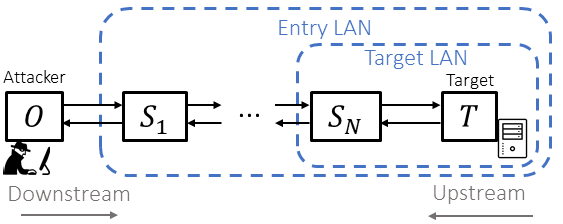
\includegraphics[width=0.6\textwidth]{images/Stepstone_final_2.png}
\caption{Depiction of an exemplary stepping-stone chain.}\label{Fig:Stepstone}
\vspace{-0.6cm}
\end{figure}

%\textcolor{red}{another popular way is using netcat}

%However, detecting that a host is used in a stepping-stone chain is a clear indication of malicious behaviour. If a stepping-stone can be identified during the attack stage, the connection can be terminated to interrupt the attack. 
Stepping-stone detection (SSD) is a process of observing all incoming and outgoing connections on a particular host $h_i$ and determining whether it is used to relay commands. This is generally done with no prior information about any other stepping-stone hosts $S_1,\dots\,S_N$ or the endpoints $O$ and $T$. A popular approach to SSD is to compare connections pairwise to identify whether they carry the same information. To avoid detection, several evasive flow transformation techniques exist that aim at decreasing observable correlation between two connections in a chain. 
 
%Once $h_i$ is known to be a stepping-stone host, further members of $\{S_1,\dots\,S_N\}$ can be traced back from $h_i$.   %This problem is closely related to the problem of tracing intruders through the Internet by following the connection chain.

%A popular approach to SSD is to compare connections pairwise to identify whether they carry the same information. A wide-spread way to achieve this is via \textit{watermarking}, an active SSD mechanism. A watermark is a unique binary string, which is usually embedded into a connection by altering the packet interarrival times. %Decoding the watermark involves capturing candidate flows that might match the water-marked flow and looking for the bits in the flow characteristics.
%Popular passive SSD methods are based on \textit{packet-correlation} and attempt to identify packets that appear in both connections. Since connections can be encrypted, this is often done by comparing sequences of interarrival times, packet sizes, and the overall number of packets in each connection.
%Anomaly-based methods aim to detect the insertion of time delays and chaff perturbations in a connection as deviations from typical TCP-behaviour to indicate of suspicious behaviour. 

%Since relaying packets over multiple hosts affects the overall connection \textit{round-trip-times} (RTTs) between the sender and receiver, another popular detection approach 

%Another prominent approach to detect stepping stones is by measuring  \textit{round-trip-times} (RTTs). The RTT of a connection is the time it takes for a packet to be sent to the receiver plus the time it takes for an acknowledgement of that packet to be received. Relaying packets affects the overall RTT.
%Since information is relayed over one or more hosts in a stepping stone chain, this has an effect on the overall RTTs which can be observed within individual connections in the chain.
%\subsubsection{Detecting Connection-Chains: A Data Mining Approach, 2010}




% typically either aims at classifying a host as a stepping stone if two connections involving this host appear to be correlated, or at classifying a connection as part of a chain if it shows characteristic side-effects of relay behaviour. Among 

%Popular SSD methods include watermarking, where the re-occurrence of an artificially embedded flow pattern  
%is to measure the \textcolor{red}{...}

%In addition, several SSD methods aim to estimate the overall length of the stepping-stone chain from the examined connection to help tracing the chain. %A traffic collection sensor is typically placed in the vicinity of the examined host to provide the necessary data. 

%A popular approach to SSD is to compare connections pairwise to identify whether they carry the same information. To avoid detection, several evasive flow transformation techniques exist that aim at decreasing observable correlation between two connections in a chain. 


\begin{itemize}

\item \textbf{Packet transfer delays/drops}: An attacker can choose to apply artificial delays to forwarded packets, or drop certain packets to cause retransmission, in order to create temporal disparity between connections. Researchers often assume the existence of a maximum tolerable delay \cite{donoho2002multiscale}.

%An easy way for an attacker to destroy flow watermarks and create temporal disparity between connections is to apply artificial random delays to forwarded packets, often also called jitter. Similarly, an attacker can choose to not forward certain packets at all and cause retransmissions. Researchers often assume the existance of a maximum tolerable delay for an attacker.

\item \textbf{Chaff perturbations}: Chaff packets do not contain meaningful content and are added to individual connections in a chain without being forwarded. Adding chaff perturbations can be used to shape the connection profile towards other traffic types. 

\item \textbf{Repacketisation}: Repacketisation is the practice of combining closely adjacent packets into a larger packet, splitting a packet into multiple smaller packets, or altering the packet content to change observed packet sizes and numbers.

%\item \textbf{Flow splitting/merging}:  An attacker can split the flow of packets to two or more connections and merge them at the target to alter the amount of packets in each connection.

\end{itemize}

In our evaluation, we set out to understand the effect of different evasive methods on detection rates. 

\section{Data generation setting}\label{Sec:Datasetcreation}

%Our goal is to simulate data that reflects the different aspects of interactive stepping-stone behaviour in a reproducible manner. For a fair and thorough evaluation, we want to cover different settings and interactions to highlight strengths and weaknesses of different SSD methods. %Furthermore, we need to generate sufficient data to effectively train some of the included methods. 


\subsection{Containerisation}

To ensure reproducibility, we rely on containerisation. A container is a standard unit of software that runs standalone in an isolated user space in order to remove platform dependencies and ensure repeatability. The use of containerisation for this project follows a traffic generation paradigm designed for machine learning, introduced by Clausen et al. \cite{clausen2019traffic}.%Compared to virtual machines, containers always start from an identical state and are highly specialized in their purpose, with each container running only a specific piece of software. 

%The advantages of containers over virtual machines enable us to easily control, modify, repeat, and scale a network of containers while emulating different network settings.  %We build our traffic generation framework on the popular containerisation platform \textit{Docker}.

%packages up code and all its dependencies so the application runs quickly and reliably from one computing environment to another. A Docker container image is a lightweight, standalone, executable package of software that includes everything needed to run an application: code, runtime, system tools, system libraries and settings.

%In contrast to standard virtual machines, containers forego a hypervisor and the shared resources are instead kernel artifacts, which can be shared simultaneously across several containers. Although this prevents the host environment from running different operating systems, containerization incurs minimal CPU, memory, and networking overhead whilst maintaining a great deal of isolation. %\cite{kolyshkin2006virtualization}. 


%. Docker enables us to script the repeated creation of steppings-stone chains within a virtual network in a scalable manner while allowing us to emulate different network settings. %\textcolor{red}{while allowing network different settings}. 

%\textcolor{red}{can we cite DetGen here?}
%\textcolor{red}{write more about Docker advantages in terms of speed and controllability}

%We build our traffic generation framework on the popular containerisation platform \textit{Docker}. %Docker allows the creation of virtualised networks to which containers can connect via a virtualised network bridge. Containers attached to the bridge network are assigned an IP address and are able to communicate with other containers on their subnetwork.

\subsection{Simulating stepping stones with SSH-tunnels and Docker}\label{Sec:Setup}

We want to capture data not only from one interaction in a fixed stepping-stone chain, but from many interactions and chains with different settings. For that, we run multiple simulations, with each simulation establishing a stepping-stone chain and controlling the interactions between host $O$ and host $T$. %A simulation and the corresponding traffic capture is in a capture-script. 

A simulation begins with the start-up of the necessary containers and ends with their takedown. We simulate host $O$, host $T$, and host $S_1,\dots,S_n$ with SSH-daemon containers. To establish a connection chain, we connect these containers via SSH-tunnels, with the first tunnel forwarding a port from host $O$ to host $S_1$, which is then forwarded to host $S_2$ by the second tunnel etc. As mentioned by Gordon Fraser \cite{pivoting2015}, this is one of the most common pivoting methods for attackers. Traffic is captured both at host $T$ and host $S_n$, which acts as the final stepping-stone in the chain.
Fig. \ref{Fig:Packetway} depicts a packet transfer via an exemplary chain. 


\begin{figure}
\centering
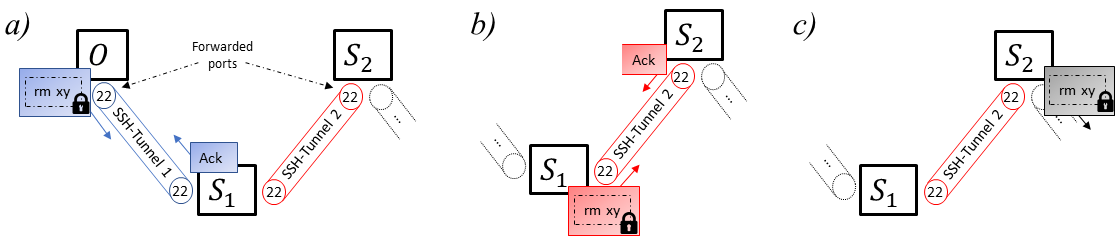
\includegraphics[width=0.9\textwidth]{images/Packetway_2.png}
\caption{Depiction of the way a command is packetised, encrypted, and travels through the different stages of the stepping-stone chain via SSH-tunnels.}\label{Fig:Packetway}
\vspace{-0.4cm}
\end{figure}

% and is most thus likely the target of a detection algorithm. 




%insert figure with one and with three stepping stones



%SSH tunnel on respective port on the starting point of the chain, tunnels to port on the next point in the chain. Finally, Refer to figure. 
\vspace{-0.6cm}
\subsubsection{Simulating interactive SSH-traffic}\label{Sec:Simulating_interactive}

In order to generate enough data instances representing interactive stepping stone behaviour, we automatised the communication between host $O$ and host $T$. For each simulation, we generate a script which passes SSH-commands from host $O$ to host $T$.%, with several measures introduced to make them realistic. 

To mimic a user's actions, we compiled a command database which consists of common commands and their usage frequency, similar to \cite{xin2006testbed}.% \cite{rossey2002lariat}. 
Commands are drawn randomly according to their usage frequency and concatenated to a script. 
Commands can either be atomic, such as "ls-la" or "pwd", or compound commands such as inputting text to a file.
%. Compound commands need additional input such as the directory and name of a specific file that is transferred, or input text to fill a file. 
Command inputs are randomised appropriately when a compound command is drawn. A scripts ends once the \textit{End}-command is drawn at random from the command catalogue. 


To simulate human behaviour that is reacting to the response from host $T$, all commands are separated by \textit{sleep}-commands for time $t$, which is drawn from a truncated Pareto-distribution. Paxson et al. \cite{paxson1995wide} have shown that interpacket spacings corresponding to typing and "think time" pauses are well described by Pareto distributions with a shape parameter $\alpha\approx 1.0$. %We use a truncated distribution capped at $10$s to avoid infinite waiting times since we already included a mechanism to end a script.


\vspace{-0.6cm}
\subsubsection{Simulating different network settings}\label{Sec:congestion}

Hosts in a stepping-stone chains can be separated by varying distances. Some may sit in the same LAN, while others may communicate via the Internet from distant geographical locations, which influences the round-trip-time, bandwidth, and network reliability. 

%Docker communication takes place over virtual bridge networks, so the throughput is far higher and more reliable than in real-world networks. %This level of speed and consistency is worrying for our purposes as packet timings will be largely identical on repeated runs of a scenario and any collected data could be overly homogeneous.
To retard the quality of the Docker network to realistic levels, we rely on the emulation tool NetEm, which allows users to artificially simulate network conditions such as high latency, low bandwidth, or packet corruption/drop \cite{hemminger2005network}.
%We apply Netem commands to the network interface of each container, which adds correlated delays to incoming and outgoing packets that are drawn from a normal distribution with mean $\mu$, variance $\sigma^2$, and correlation $\rho_1$. We furthermore apply correlated packet loss and corruption drawn from a binomial distribution with probability $p$ and correlation $\rho_2$. Lastly, we apply an overall limit $B$ on the bandwidth of container network interfaces.
%To allow for different types of host separation, 
We set the network settings and bandwidth limit for each host container individually before each simulation to allow hosts to experience different settings.
%, and draw each of the given parameters from a suitable distribution. This 
%which allows for some hosts to experience very fast and reliable communication while others experience more congested communication. %\textcolor{red}{(should I specify which one for each? Seems a bit much...)} %before each \textcolor{red}{run} to allow for a good amount of variation in the generated data.
%We store the drawn parameters along with the collected traffic for each simulation to include the effect of network congestion in the evaluation. 

%providing us with the flexibility to set each container's network settings uniquely. 




%This script randomizes the values of each parameter, such as packet drop rate, bandwidth limit, latency, ensuring that every run of a scenario has some degree of network randomization if desired.


\subsection{Evasive tactics}

\subsubsection{Adding transfer delays}\label{Sec:delays_desc}

To simulate evasive behaviour, we add transfer delays to forwarded packets. This method, often called \textit{jittering}, can destroy time-based watermarks in packet flows and help decrease observable correlation between two connections. The delays are added using NetEm. We draw delays from a uniform distribution, covering the interval $[0,\delta_D]$. This particular choice has been suggested by Padhye et al. \cite{padhye2010evading} in order to mimic the interarrival distributions of streaming services. The value of $\delta_D$ is fixed before each simulation and can be varied to allow for different degrees of packet jittering. We explore values for $\delta_D$ up to $1500$ ms, with values above leading to unstable communication. Results in Section \ref{Sec:Results} show that this is enough to render watermarking methods and most flow correlation methods obsolete.

%\textcolor{red}{insert citation} suggested to use significantly longer packet delays of several seconds to request packets and their answers in order to decrease temporal correlation between active periods in two connections.
%As pointed out by Donoho et al. \cite{donoho2002multiscale}, excessively long delays often lead to difficulties in the TCP-protocol due to the significant increase of packet reordering and response time-outs. % while flow decorrelation can be achieved more effectively by using chaff perturbations.


\vspace{-0.6cm}
\subsubsection{Adding chaff perturbation}\label{Sec:chaff_desc}

We insert chaff packets without actual information to individual connections in the chain using a Netcat client. %The inserted chaff packets do not contain actual information and act as noise to decorrelate individual connections in the chain. 
To add and filter packets in a connection, we open additional ports in each SSH-tunnel that are however not forwarded through the entire chain. %This means that each chaff packet only appears in the connection it was inserted to, making the chaff perturbation in two different connections independent of each other. 
%We then use a NetCat client containers to send and receive packets on the additional ports in both directions. %Figure \textcolor{red}{...} depicts this setup. 
%\textcolor{red}{add reference} to send data to both ports from either direction and collect it at the other side. 
Padhye et al. \cite{padhye2010evading} suggest to generate chaff that mimics the flow characteristics of streaming services to both spread the added perturbations evenly across the connection and increase the difficulty of detecting the perturbation itself.
For this, packet sizes are drawn from a truncated Lognormal-distribution with mean $\mu_C$, while transmission intervals are drawn from a uniform distribution that covers the interval $[\delta_C/2,\delta_C]$ to mimic a constant packet flow. By adjusting $\delta_C$, we can control the amount of chaff sent.

\vspace{-0.6cm}
\subsubsection{Repacketisation}% and Flow splitting/merging}

%From an attackers perspective, a benefit of using SSH-tunnels is that packets are not simply forwarded, but a tunnel acts as an independent encrypted TCP-connection along with independent packet confirmations and repacketisation.

By design, SSH-tunnels perform repacketisation along with re-encryption and independent packet confirmations.
%Flow splitting is currently not addressed by existing methods, which is why we did not include this tactic in our implementation.
%None of the methods we encountered are currently capable of dealing with flow splitting or merging. We therefore did not implement this tactic as the results would be uninformative.


\begin{figure}
\centering
\includegraphics[width=0.75\textwidth]{images/Docker_framework.png}
\caption{Depiction the simulation setup for each host in the chain.}\label{Fig:Simulation_setup}
\vspace{-0.6cm}
\end{figure}

%Fig. \ref{Fig:Simulation_setup} depicts the interplay of the different containers in our simulation.


%\subsection{HTTP-interactions}
 
%In order to provide an additional, different type of interaction between the \textcolor{red}{starting point} and \textcolor{red}{end point}, we directed HTTP traffic over the stepping stone chain. Here, the starting point hosts Scrapy, a web crawling service \textcolor{red}{insert citation}, that surfs the 1 million most popular website by clicking links on them. The requests are sent over the stepping stone chain to the web. 

%This type of traffic is not meant to necessarily represent realistic stepping stone behaviour, but to provide an additional source of interactive traffic that differs substantially from SSH in order to test detection methods from another angle.




%\begin{tabular}{r|cccc|cccc}
%\multicolumn{1}{r|}{ }&\multicolumn{4}{c|}{SSH}&\multicolumn{4}{c}{HTTP}\\
%bla& no pert.&var. delays&var. chaff&delay\&chaff & no pert.&var. delays&var. chaff&delay\&chaff \\
%\end{tabular}

%\begin{tabular}{r|cccc}
%\multicolumn{1}{r|}{ }&\multicolumn{4}{c|}{SSH}&\multicolumn{4}{c}{HTTP}\\
%SSH 1 node& no pert.&var. delays&var. chaff&delay\&chaff \\
%HTTP 1 node& no pert.&var. delays&var. chaff&delay\&chaff \\
%SSH 3 node& no pert.&var. delays&var. chaff&delay\&chaff \\
%HTTP 1 node& no pert.&var. delays&var. chaff&delay\&chaff \\
%\end{tabular}


 
%\cite{sommer_outside_2010}

%\subsection{Regular traffic congestion}

%Packet transmission in Docker's virtual network is almost instantaneous and not subject to transmission errors. 
%To emulate realistic traffic as close as possible, we add emulated traffic congestion in the form of packet delivery delays and packet losses. These are implemented between individual hosts using tc-netem.

%Delays are added to incoming and outgoing packets on each host individually, and are drawn from a normal distribution. The mean and standard deviation are drawn before each simulation for each host.

\section{Evaluation data}\label{Sec:Evaldata}

%The quality of both the stepping-stone and background data is crucial for a fair evaluation. 

We want to look at a variety of attack scenarios to highlight the strengths and weaknesses of different SSD approaches. We created three main attack datasets that contain different forms and amounts of evasive behaviour, and a smaller dataset to highlight the influence of different chain lengths. 

To present a valuable false positive test, we provide three datasets with benign background traffic. The first contains general real-world traffic, while the second and third contain benign data that bears similar traffic characteristics as the generated attack data. %Furthermore, we need to generate sufficient data to effectively train some of the included methods. 

%We now describe our data assembly in more detail.

\subsection{Stepping-stone data}

%We generate stepping-stone data using the setup described in Section \ref{Sec:Datasetcreation}. 
We create our main datasets using a chain of four stepping-stones $S_1, S_2, S_3$, and $S_4$. We subdivide into three datasets: We first capture data without transfer delays and chaff perturbations in \textbf{dataset BA} (\textbf{b}aseline \textbf{a}ttack). We then capture data once with added transfer delays with varying $\delta_D$ to control delays in \textbf{dataset DA} (\textbf{d}elay \textbf{a}ttack), and once with added chaff perturbations of varying $\delta_C$ in \textbf{dataset CA} (\textbf{c}haff \textbf{a}ttack). Each dataset contains 30.000 connection pairs.
%Lastly, we capture data with delays and chaff added simultaneously, with both varying $\delta_D$ and $\delta_C$.
We furthermore create a smaller \textbf{dataset CL} (\textbf{c}hain \textbf{l}ength) with differing numbers of stepping-stones (1,3,5, and 8 jumps) without transfer delays and chaff perturbations.% to evaluate this effect on RTT-based methods. %For every jump, we generated 1.000 connection pairs.

%For all datasets, we randomise network settings. In Section \ref{Sec:InfluenceNetwork}, we examine the effect of extreme network settings on detection rates. 
%Table \ref{Tab:MalData} provides a summary of the connection pair numbers in each part of the dataset.
%\begin{table}
%\centering
%\begin{tabular}{l|r}
%4 jumps&\# connection pairs \\ \hline
%No evasion& 30.000\\ \hline
%Delays& 30.000 \\ \hline
%Chaff&30.000 \\ \hline
%\hline
%1 jump& 1.000\\ \hline
%3 jump& 1.000 \\ \hline
%5 jump& 1.000 \\ \hline
%8 jump& 1.000 \\ \hline
%\end{tabular}
%\caption{Number of connection pairs in each part of the stepping-stone dataset.}\label{Tab:MalData}
%\end{table}

%Table \ref{Tab:Stepstone_data} depicts the number of connection pairs included in each dataset.

%\begin{table}
%\centering
%\begin{tabular}{r|c|c|c|c}
%\multicolumn{1}{r|}{ }&\multicolumn{4}{c|}{SSH}&\multicolumn{4}{c}{HTTP}\\
%nodes & no evasion & delays & chaff & delays\& chaff \\
%\hline
%1-node & 10.000 & 10.000 & 10.000 & 10.000 \\
%4-node & 10.000 & 10.000 & 10.000 & 10.000 \\
%\end{tabular} 
%\caption{}\label{Tab:Stepstone_data}
%\end{table}

 
\subsection{Benign data}

%We need to provide a realistic background of benign data that reflects the heterogeneous nature of regular network traffic, both for evaluation of false positives and for the training of ML-based methods.

We include real-world traffic traces, taken from the \textbf{CAIDA} \textit{2018 Anonymized Internet Traces} dataset \cite{CAIDA2018}, as overall background traffic. This data contains traces collected from high-speed monitors on a commercial backbone link, and is often used for research on the characteristics of Internet traffic.%, including application breakdown, security events, geographic and topological distribution, flow volume and duration.
%\textcolor{red}{insert citation and description}.


%The CAIDA dataset provides suitable general background traffic. 
To sufficiently test for false-positive, we also need to include benign traffic that has similar characteristics to the attack traffic and was generated in a similar network environment. We created a set of interactive SSH-connections that communicate directly between the client and the server without a stepping-stone. We follow the same procedure as described in Section \ref{Sec:Simulating_interactive}.% with the same randomised network congestion settings as described in \ref{Sec:congestion}. We then proceed to pair connections by random.

%Additionally, we include a third type of benign traffic . 
Since we generate perturbations with multimedia streams characteristics, we additionally want to test for false-positives against actual multimedia stream traffic. For that, we captured traffic from a Nginx-server streaming randomised video to a client. %Video content is generated randomly from a set of video files and multiple values for the streaming quality are used.
%The server and client are hosted in the same virtual Docker network with randomised network congestion settings. 
%Again, we pair connections by random, but we ensure that the direction of the streams forms a chain. 
%However, for each pair the direction of the transfer has to be either to or from the common host to either resemble a client requesting two videos or a server sending to videos.


% according to the following ratios:

%\begin{table}
%\centering
%\begin{tabular}{l|r}
%&\# pairs \\ \hline
%CAIDA& 60.000\\ \hline
%SSH& 20.000 \\ \hline
%multimedia& 20.000 \\ \hline
%\end{tabular}
%\caption{Ratio of traffic in the benign dataset.}\label{Tab:Benigndata}
%\end{table}


%\begin{table}
%\centering
%\begin{tabular}{l|l|l|l}
%& Label  &Nr. of conn. & Purpose\\ \hline
%\multirow{5}{*}{Attack data}& set BA & 30.000& \makecell[l]{Baseline attack data without\\evasion tactics} \\ \cline{2-4}
%						& set DA & 30.000& Inclusion of delays with varying %$\delta_D$ \\ \cline{2-4}
%						& set CA & 30.000& Inclusion of chaff with varying %$\delta_C$ \\ \cline{2-4}
%						& set CL & 40.000& \makecell[l]{Data from chains of different\\lengths,  no evasion tactics} \\ \hline
%\multirow{5}{*}{Background data}&CAIDA & 60.000& General background data \\ \cline{2-4}
%							&SSH & 20.000& \makecell[l]{Background data %similar to\\attack commands} \\ \cline{2-4}
%							&Multim.& 20.000& \makecell[l]{Background data similar to\\chaff perturbations} \\ \hline
%\end{tabular}
%\caption{Summary of different components in our evaluation data.}\label{Fig:Datasim}
%\end{table}


\begin{table}
\centering
\begin{tabular}{l|l|l|l}
& Label  &Nr. of conn. & Purpose\\ \hline
\multirow{4}{*}{Attack data}& set BA & 30.000& Baseline attack data without evasion tactics \\ \cline{2-4}
						& set DA & 30.000& Inclusion of delays with varying $\delta_D$ \\ \cline{2-4}
						& set CA & 30.000& Inclusion of chaff with varying $\delta_C$ \\ \cline{2-4}
						& set CL & 40.000& Data from chains of different lengths,  no evasion tactics \\ \hline
\multirow{3}{*}{Background data}&CAIDA & 60.000& General background data \\ \cline{2-4}
							&SSH & 20.000& Background data similar to attack commands \\ \cline{2-4}
							&Multim.& 20.000& Background data similar to chaff perturbations \\ \hline
\end{tabular}
\caption{Summary of different components in our evaluation data.}\label{Fig:Datasim}
\vspace{-0.6cm}
\end{table}



We merge the three datasets to create our benign background dataset, with the CAIDA part containing 60.000 connection pairs, while the other two each contain 20.000 connection pairs. 
The amount of SSH traffic and multimedia streams in this setting is inflated from a realistic setting (up to $0.2\%$ of flows for SSH and up $3\%$ for video streaming \cite{velan2016network}) to highlight the strengths and drawbacks of SSD methods, which we consider in the evaluation. %Nevertheless, SSH and especially video streaming represent a significant proportion of overall network traffic (up to $0.2\%$ of flows for SSH and up $3\%$ for video streaming according to Velan et al. in 2016 \cite{velan2016network}), and need to generate low false-positives for an SSD-method to be operational. 
In Section \ref{Sec:FPana}, we analyse false-positives for each dataset individually.
Table \ref{Fig:Datasim} summarises the different parts in our evaluation data.

%but we believe that this setting is more suitable to highlight the strengths and drawbacks of SSD methods. In the evaluation, we will also state individual false positives for each of the three datasets to indicate which type of traffic present the biggest challenge for the selected SSD methods. 

%\begin{figure}
%\begin{tikzpicture}[
%    grow=right,
%    level 1/.style={sibling distance=6cm,level distance=3.2cm},
%    level 2/.style={sibling distance=1.8cm, level distance=4.5cm},
%    edge from parent/.style={very thick,draw=blue!40!black!60,
%        shorten >=5pt, shorten <=5pt},
%    edge from parent path={(\tikzparentnode.east) -- (\tikzchildnode.west)},
%    kant/.style={text width=2cm, text centered, sloped},
%    every node/.style={text ragged, inner sep=2mm},
%    punkt/.style={rectangle, rounded corners, shade, top color=white,
%    bottom color=blue!50!black!20, draw=blue!40!black!60, very
%    thick }
%    ]
%
%\node[punkt, text width=5.5em] {\textbf{Evaluation data}}
%    %Lower part lv1
%    child {
%        node[punkt] [rectangle split, rectangle split, rectangle split parts=2,
%         text ragged] {
%            \textbf{Benign data}
%                  \nodepart{second}
%            100.000 connect.
%        }
%		child {
%            node [punkt, rectangle split, rectangle split parts=2]{
%                \textbf{Video streaming}
%                \nodepart{second}
%                similar to chaff, 20.000
%            }
%            edge from parent
%                node[kant, above] {}}
%		child {
%            node [punkt,align=left, rectangle split, rectangle split parts=2]{
%                \textbf{interactive SSH}
%                \nodepart{second}
%                similar to attack\\ commands,  20.000
%            }
%            edge from parent
%                node[kant, above] {}}
%        child {
%            node [punkt, rectangle split, rectangle split parts=2]{
%                \textbf{CAIDA}
%                \nodepart{second}
%                gen. background, 60.000
%            }
%            edge from parent
%                node[kant, above] {}}
%        edge from parent
%            node[kant, below, pos=.6] {}
%    }
%    %Upper part, lv1
%    child {
%        node[punkt, rectangle split, rectangle split parts=2] {
%	\textbf{SS data}
%                \nodepart{second}
%                94.000 connect.
%        }
%		child {
%            node [punkt, rectangle split, rectangle split parts=2]{
%                \textbf{set CL}
%                \nodepart{second}
%                mult. jumps, 4.000
%            }
%            edge from parent
%                node[kant, above] {}}
%        child {
%            node [punkt, rectangle split, rectangle split parts=2]{
%                \textbf{set CA}
%                \nodepart{second}
%                chaff, 30.000
%            }
%            edge from parent
%                node[kant, above] {}}
%		child {
%            node [punkt, rectangle split, rectangle split parts=2]{
%                \textbf{set DA}
%                \nodepart{second}
%                delays, 30.000
%            }
%            edge from parent
%                node[kant, above] {}}
%         child {
%            node [punkt,rectangle split, rectangle split,
%            rectangle split parts=2] {
%                \textbf{set BA}
%                \nodepart{second}
%                no evasion, 30.000
%            }
%            edge from parent
%                node[below, kant,  pos=.3] {}}
%            edge from parent{
%                node[kant, above] {}}
%    };
%\end{tikzpicture}
%\caption{Summary of different components in our evaluation data.}\label{Fig:Datasim}
%\end{figure}

\subsection{Evaluation methodology}


%We collect packets to connections according to the usual 5-tuple consisting of \{Src. IP, Dst. IP, Src. port, Dst. port, IP protocol\}. We select and pair TCP-connections at random to make %100.000 connection pairs.

%Different approaches require different amounts of packets to make predictions. 
To create a fair playing field for the selected SSD methods, we only look at connections that exchange more than 1500 packets and exclude shorter connections from both the data.
%compiled background dataset and the attack dataset. 
The number of packets necessary for detection should ideally be a low possible to enable early detection. The chosen number of 1500 packets seems like a suitable minimal limit since all of the selected methods are designed to make successful detection with 300-1500 packets.  Furthermore, there were no connections with less packets in the stepping-stone dataset. %\textcolor{red}{add validation about how this is sufficient for all approaches?}.
%The first 1500 packets are then passed to each SSD method to make a prediction.

%The initialisation and takedown of the SSH-tunnels usually follows a distinct pattern that can be learned and consequently boost detection rates for ML-based methods. Since this pattern is not necessarily representative of actual stepping-stone behaviour, we remove the first and last thirty packets in the attack connections. %If necessary, we also remove the last thirty packets to avoid the same issue for connection closures. 

%\subsection{Evaluation methods}

%All of the above presented methods classify individual connections or pairs of connections as malicious or benign. 
True stepping stone connections are rare compared to benign ones, making their detection an imbalanced classification problem. An appropriate evaluation measure for imbalanced data are false positive and false negative rates as well as the \textit{Area-under-ROC-curve} (AUC) for threshold-based methods.


\section{Selected SSD methods and Implementation}\label{Sec:Selection}

%The main contribution of this work is to offer a modern evaluation of the current state of SSD methods. 
A range of underlying techniques exist for SSD, and we try to include approaches from every area to create an informative overview and highlight strengths and weaknesses. 
We surveyed publications to create a collection of SSD methods. We started with the publications from surveys \cite{shullich2011survey,wang2018research}, and then added impactful recent publications found via Google Scholar\footnote{keywords ``connection'', ``correlation'' ``stepping-stone'', ``detection'', ``attack'', ``chaff perturbation''}.
% from 2018 and 2011, mentioned in Section \ref{Sec:Relatedwork}. We expanded this collection via finding publications that cited these papers. Lastly, we found publications by browsing Google Scholar with different combinations of the keywords ``connection'', ``correlation'' ``stepping-stone'', ``detection'', ``attack'', ``chaff perturbation''. Our final collection contained 60 publications. 
From here, we selected approaches based on the following criteria:


\begin{enumerate}
\item The achieved detection and false positive rates claimed by the authors,
\item and whether the model design shows robustness against any evasion tactics as claimed by the authors.
\item We always selected the latest versions if a method has been improved by the authors.
\end{enumerate}


Table \ref{Tab:Summary} contains a summary of the included methods. Especially for traditional packet-correlation as well as robust watermarking and anomaly-based methods, there has been little developments since the early 2010s.
We labelled each method to make referring to it in the evaluation easier.

\begin{table}
\centering
\begin{tabular}{l|c|c|c|c|c}
Category & Approach & TP & FP & Robustness & Label\\ \hline

Packet-corr. & Yang, 2011 \cite{yang2011correlating} & $100\%$ & $0\%$& jitter/$<80\%$ chaff & PContext\\ \hline

\multirow{2}{*}{Neural networks} & Nasr, 2018 \cite{nasr2018deepcorr} &$90\%$ & $0.0002\%$& small jitter & DeepCorr\\ \cline{2-6}
 
 & Wu, 2010 \cite{wu2010neural} & 100\% & 0\% & - & WuNeur\\ \hline
 
\multirow{2}{*}{RTT-based} & Yang, 2015 \cite{yang2015rtt}& \multicolumn{2}{c|}{not provided} & $50\%$ chaff &RWalk\\ \cline{2-6}

& Huang, 2016 \cite{huang2016detecting} & $85\%$ & $5\%$ & - & Crossover\\ \hline
 
\multirow{2}{*}{Anomaly-based} & Crescenzo, 2011 \cite{di2011detecting} & $99\%$ & $1\%$ & jitter/chaff &Ano1\\ \cline{2-6}

& Huang, 2011 \cite{huang2011detecting,ding2013detecting} & $95\%$ & $0\%$ & $>25\%$ chaff/ $>0.2$s jitter &Ano2\\ \hline

Watermarking & Wang, 2011 \cite{wang2010robust} & $100\%$ & $0.5\%$ & $<1.4$s jitter & WM\\ \hline
\end{tabular}
\caption{Summary of included SSD-methods along with the claimed true positive and false positive rates and evasion robustness by the corresponding authors. We added labels to each method for later reference.}\label{Tab:Summary}
\vspace{-0.6cm}
\end{table}


%We believe that these criterias are sufficient to 

%Researchers have so far proposed two main approaches: passive monitoring and active perturbation. In the latter

%\subsubsection{Detecting Connection-Chains: A Data Mining Approach, 2010}


%TPR 100\% and FPR 0\%
%\vspace{-0.3cm}

\subsubsection{PContext, 2011}

Yang et al. \cite{yang2011correlating} compare sequences of interarrival times in connection pairs to detect potential stepping-stone behaviour. For that, the contextual distance of a packet is defined as the packet interarrival times around that packet. %The respective contextual distance between packets is estimated using the Pearson correlation. %Packets with high correlation are defined as `matched', and two connections are classified as relayed if the ratio of matched packets exceeds a threshold. 
The authors focus on \textit{Echo}-packets instead of \textit{Send}-packets to resist evasion tactics.%, as the sending of \textit{Echo}-packets is subject to more constraints and less easy to manipulate.
The authors evaluate their results with up to $100\%$ chaff ratio with $100\%$ detection rate.

\vspace{-0.6cm}
%\subsection{Neural networks}

%The authors present two networks to identify stepping stones. 
%The first method uses eight packet variables of an individual packet as input to predict the number of stepping-stones.




\subsubsection{WuNeur, 2010}

%A notable initial example of neural network applications to SSD came from Wu et al. \cite{wu2008performance}, and which was later improved by the authors \cite{wu2010neural}.
%however, the authors concluded that the achieved results did not improve existing detection rates. but no good results, better in Neural networks-based detection of stepping-stone intrusion.
Wu et al. \cite{wu2010neural} propose a neural network model based on sequences of RTTs%. For this, a packet matching algorithm is used to compute RTTs, which are then fed as a fixed-length sequence
, which are fed into a feed-forward network to predict the downstream length of the chain. The network itself only contains one hidden layer and achieves good results only if RTTs are small, i.e. when the stepping-stone chain is completely contained within one LAN-network.

\vspace{-0.6cm}
\subsubsection{DeepCorr, 2018}

Nasr et al. \cite{nasr2018deepcorr} train a deep convolutional neural network to identify connection correlation from the interarrival times and packet sizes in each connection. The trained network is large with over 200 input filters, and consists of three convolutional and three feed-forward layers. %The trained model was initially applied to a dataset of Tor-connections.%, where the authors achieved strong results. 
On stepping-stones, the authors achieve a $90\%$ detection rate with $0.02 \%$ false positives. 

\vspace{-0.6cm}
\subsubsection{RWalk, 2015}


Yang et al. \cite{yang2015rtt} combine packet-counting methods and RTT mining methods to improve detection results from \cite{yang2007mining}. 
%A widely-used approach is to compare the number of incoming packets in one connection with the number of outgoing packets in another connection to determine if the pair represents a stepping stone relay. However, the insertion of chaff can separate these numbers substantially.
%The authors improve widely-used packet-counting methods to 
THe model resists chaff perturbation by estimating the number of round-trips in a connection via packet-matching and clustering to determine if the connection is being relayed.
%To resist intruders evasion, the authors propose to use the 
%Packet pairs representing a round-trip for each connection are estimated using a combination of packet matching and clustering, and counted as $N_{in}$ and $N_{out}$. %The authors then claim that the value of $N_{in}-N_{out}$ is only bounded if the two connections are relayed.

\vspace{-0.6cm}
\subsubsection{C-Over, 2016}

Huang et al. \cite{huang2016detecting} use the fact that in long connection chain, the round-trip-time of a packet may be longer than the intervals between two consecutive keystrokes. %Normally after sending a request packet, a client will wait for the server response before sending another request. 
%TCP/IP allows a client to send a limited number of packets to the server without having to wait for the response. 
This will result in cross-overs between request and response, which causes the curve of sorted upstream RTTs to rise more steeply than in a regular connection. %A stepping stone is detected if the maximum increase in the curve exceeds a threshold. 
%The authors do not state overall detection rates.
%a universal threshold value and instead suggest a method to estimate the appropriate value for a given setting.
%Detecting Stepping-Stone Intruders by Identifying Crossover Packets in SSH Connections

%.

%.

%RTT-based Random Walk Approach to Detect Stepping-Stone Intrusion 

%Detecting Stepping-Stone Intruders with Long Connection Chains? 2009


\vspace{-0.6cm}
\subsubsection{Ano1, 2011}

Crescenzo et al. \cite{di2011detecting} have proposed an anomaly-based methods to detect time delays and chaff perturbations in a selected connection. 
Packet time-delays are detected if RTTs exceed a threshold, while chaff detection compares the similarity of downstream with upstream sequences.%, and a causality-based method verifies that the number of ON-intervals in upstream and downstream direction match.
The authors claim detection for chaff ratios 25\% or more, and for delays introduced to up to 70\% of all packets.

%. It estimates the RTT of a connection, and then flags acknowledgement packets if their response-time exceeds (RTT+$\delta_{RT}$). The authors claim that an attacker would have to impose delays on more than 70\% of all packets to evade this method.
%\item The edit-distance based method is comparing packet sequences ON-OFF intervals in upstream and downstream in a connection, which should be similar to each other in a benign connection. The assumption is that chaff insertation is often independent in the two directions, leading to dissimilarities. 
%\item The causality-based method is verifying that the number of ON-intervals in upstream and downstream direction match each other to detect chaff.
%\end{enumerate}
\vspace{-0.6cm}
\subsubsection{Ano2, 2011/2013}
Huang et al. \cite{huang2011detecting,ding2013detecting} proposed an anomaly-based method to detect chaff and delay perturbations since interarrival times in regular connections tend to follow a Pareto or Lognormal distribution, which chaffed connections supposedly do not. %The authors perform a statistical test whether packets in a connection follow these distributions.% in order to classify them into normal and chaffed connections.
%describing the fit of interarrival times to these distributions that is used to classify connections into normal and chaffed connections.
%A similar approach from the same authors  is directed towards the detection of packet jittering.
The authors state $95\%$ detection rate at $50\%$ chaff ratio and more while retaining zero false positives using a small set of interactive SSH stepping-stone connections.
% generate a small set of chaffed interactive SSH stepping-stone chains, where they achieve a $95\%$ detection rate on connections which are subject to a $50\%$ chaff ratio while retaining zero false positives. For lower chaff ratios, the detection rate decreases significantly. 

% Afterwards, the goodness-of-fit is tested using two statistical tests, which yield a \textit{disagreement-of-fit score}. If this disagreement score exceeds a threshold, which was determined from a set of know regular connections, the connection is seen as being subject to chaff perturbations. The authors generate a small set of chaffed interactive SSH stepping-stone chains, where they achieve a $95\%$ detection rate on connections which are subject to a $50\%$ chaff ratio while retaining zero false positives. For lower chaff ratios, the detection rate decreases significantly. 

%A similar approach from the same authors \cite{ding2013detecting} is directed towards the detection of packet jittering. However, instead of estimating a disagreement-of-fit score, the authors use the estimated distribution parameters as input to train a support vector machine. 


%A watermark is simply an unique binary string. The process of embedding one bit of this string consists of changing some property, usually packet interarrivals, of a traffic flow such that the change represents a bit. Decoding the watermark involves capturing candidate flows that might match the water-marked flow and looking for the bits in the flow characteristics. The bits of the watermark should have enough redundancy to ensure that they are decoded correctly with high probability.
\vspace{-0.6cm}
\subsubsection{WM, 2010}
Watermarking typically yields very low false-positives for connection correlation. %However, as found by \cite{iacovazzi2016network}, usually not very robust against timing and chaff perturbation attacks. 
Wang et al. \cite{wang2010robust} provide an approach that offers at least some resistance against timing perturbations. The authors assume some limits to an adversary's timing perturbations, such as a bound on the delays.%, divide a sequence of packets into pairs, whose interarrival time is perturbed using a new watermarking function. %The introduced watermark is invisible for third-parties, and % and can be decoded in packet sequences longer than 600 packets using $m=12$ when $s=400ms$. 
The authors state $100\%$ TP with $0.5\%$ FP with resistance against timing perturbations of up to $1.4s$.

%two groups of length $m$, and match packets from both groups into pairs. Each pair interarrival time is then perturbed using a watermarking function in dependence of an overall perturbation value $s$. 
%The introduced watermark is invisible for third-parties and can be decoded in packet sequences longer than 600 packets using $m=12$ when $s=400ms$. The authors achieve $100\%$ TP with $0.5\%$ FP and claim resistance against timing perturbations of up to $1.4s$.


%Iacovazzi et al. \cite{iacovazzi2016network} found that flow watermarking is done overwhelmingly through 



%The false positive rate is defined as
%
%\begin{align*}
%\frac{\text{number of benign connections classified as malicious}}{\text{overall number of benign connections}},
%\end{align*}
%
%while the false negative rate is defined as
%
%\begin{align*}
%\frac{\text{number of malicious connections classified as benign}}{\text{overall number of malicious connections}}.
%\end{align*}
%
%Some methods additionally try to predict the length of the stepping stone chain.
%
%Write that we grant each method enough packets

%\subsection{Implementation of selected approaches}

%In order to evaluate the above selected method on our generated data, we had to

%We reimplemented all selected algorithms in Python and PyTorch according to the steps and design described in the corresponding publications. %We implemented all methods in Python, and PyTorch if necessary. %To overcome unclear points or adjust to the new setting, we had to make a small number of judgement calls, the most important of which we mention here for completeness:
%For all methods, we either varied the classification threshold for AUC calculation, or estimated it to yield a specific false positive rate across all methods. For anomaly-based methods, we had to estimate multiple thresholds, for which we found the optimal combination via grid-search. %We found appropriate values that yield the required FP rate and maximise the detection rate over all datasets via grid-search optimisation.
%For the WM approach, we set the quantization step size $s=0.4$s, and the redundancy number $m=11$ to consistently embed the watermark in the first 1500 packets. These values were also used by the authors.

%Both DeepCorr and WuNeur are machine-learning based algorithms that require training. Since DeepCorr is a large model and requires a lot of training data, we train it using $80$\% of the evaluation data. WuNeur is sensitive to differing chain lengths, which is why we use 1000 connection pairs from each dataset BA, DA, CA, and CL, as well as 6000 connection pairs from the training data. %We train each method for 500 epochs. 


%\textcolor{red}{add short description how we trained approaches}

\section{Results}\label{Sec:Results}


\subsection{Data without evasion tactics}

\begin{knitrout}
\definecolor{shadecolor}{rgb}{0.969, 0.969, 0.969}\color{fgcolor}\begin{figure}
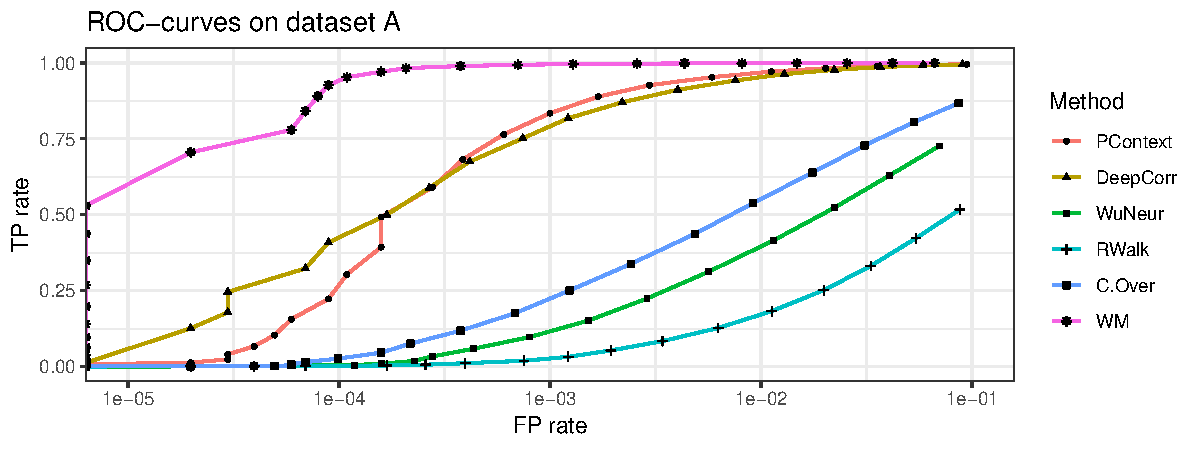
\includegraphics[width=\maxwidth]{figure/Noevasion_4nodes-1} \caption[ROC-curves for different SSD methods on dataset BA (no evasive tactics)]{ROC-curves for different SSD methods on dataset BA (no evasive tactics). Anomaly-based methods are excluded.}\label{fig:Noevasion_4nodes}
\end{figure}


\end{knitrout}


First, we look at the detection rates for traffic from stepping-stones that did not use any evasive tactics, i.e. $S_1,\dots,S_4$ are only forwarding commands and responses. The successful detection of this activity with low false-positives should be the minimum requirement for any SSD method. Since anomaly-based approaches aim to only detect evasive behaviour, we exclude them from this analysis. 

\begin{table}
\centering
% latex table generated in R 3.5.3 by xtable 1.8-3 package
% Thu Aug 13 15:10:05 2020
\begin{tabular}{l|r|r|r|r|r|r}
  \hline
 & PContext & DeepCorr & WuNeur & RWalk & C-Over & WM \\ 
  \hline
AUC & 0.998 & 0.997 & 0.938 & 0.853 & 0.965 & 0.9998 \\ 
   \hline
\end{tabular}

\caption{AUC-scores for different methods on stepping-stone data without evasive tactics.}\label{Tab:dfAUC}

\vspace{-0.6cm}
\end{table}

Fig. \ref{fig:Noevasion_4nodes} depicts the calculated ROC-curves, which plot the true positive rate against the false positive rate for varying detection thresholds. Table \ref{Tab:dfAUC} depicts the overall AUC-scores.


%\textcolor{red}{insert NN approaches trained without noise?}

Unsurprisingly, the watermarking method achieves high detection results with very low false-positives. Both the PContext and DeepCorr models start to yield good detection results of around $80\%$ at a FP rate lower than $0.1\%$, with the PContext method slightly outpacing the DeepCorr method. 
RTT-based methods seem to not perform as well compared to the other included methods. Overall, the observed ROC curves seem to be in agreement with the stated detection rates of the selected methods except for RWalk. %\textcolor{red}{check this again}.



%A possible explanation could be that each 

\subsection{Delays}

We now consider the effect of transfer delays added by the attacker to packets on the detection rates. For that, we pick detection thresholds for each SSD methods corresponding to a FP rate of $0.4\%$ as most methods are able to achieve at least moderate detection results at this rate. 
We look at delays added to only to outgoing packets on $S_4$, the last stepping stone in the chain. Fig. \ref{fig:Delaydetection} depicts evolution of detection rates in dependence of the maximum delay $\delta_D$.


%\textcolor{red}{consider two types of delays?}

\begin{knitrout}
\definecolor{shadecolor}{rgb}{0.969, 0.969, 0.969}\color{fgcolor}\begin{figure}
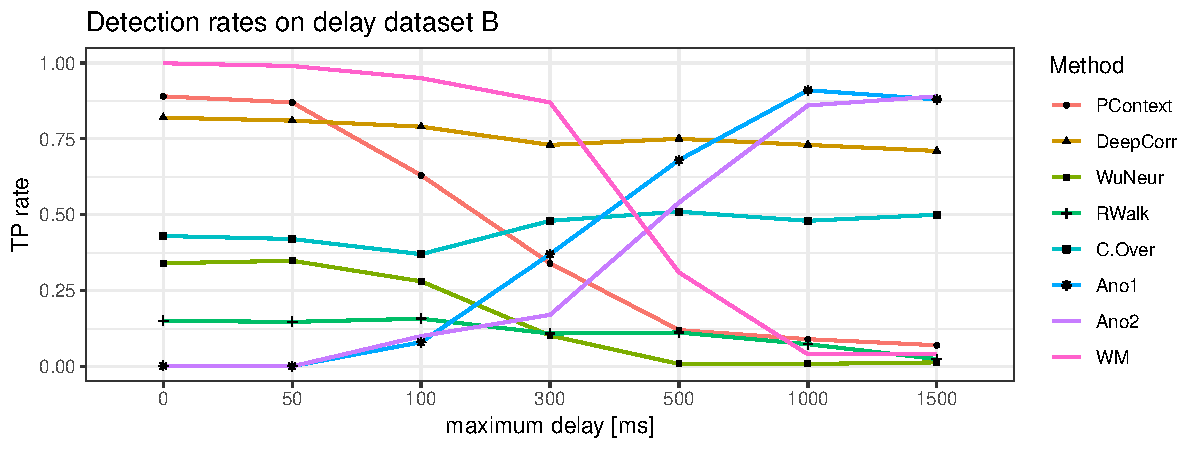
\includegraphics[width=\maxwidth]{figure/Delaydetection-1} \caption[Detection rates in dependence of $\delta_D$ for different methods on dataset DA with a fixed FP rate of $0.4\%$]{Detection rates in dependence of $\delta_D$ for different methods on dataset DA with a fixed FP rate of $0.4\%$.}\label{fig:Delaydetection}
\end{figure}


\end{knitrout}

As visible, both anomaly-based methods are capable of detecting added delays relatively reliably above a certain threshold. Furthermore, both the detection rates of DeepCorr and the RTT-based C-Over only decrease slightly under the influence of delays. Detection rates for all other methods decrease significantly to the point where no meaningful predictions can be made. This is also reflected by the AUC-scores for traffic with $\delta_D=1000ms$, given in Table \ref{Tab:AUCdelays}.

While the WM method is robust against transfer delays up to $\delta_D=500$ms, this value is smaller than the one claimed by the authors. This might however be a result of the slightly smaller quantisation step size that we used. It is surprising that the PContext method shows only little robustness against transfer delays, which contradicts the authors claims, potentially due to the incorrect assumption that relying on \textit{Echo}-packets are not subject to transfer delays.
%, since we also successfully apply delays to them while additional non-delayed \textit{Echo}-packets are generated by the tunnels. 


\begin{table}
\centering
% latex table generated in R 3.5.3 by xtable 1.8-3 package
% Thu Aug 13 15:10:09 2020
\begin{tabular}{l|r|r|r|r|r|r|r|r}
  \hline
 & PContext & DeepCorr & WuNeur & RWalk & C-Over & Ano1 & Ano2 & WM \\ 
  \hline
AUC & 0.638 & 0.995 & 0.613 & 0.641 & 0.952 & 0.997 & 0.996 & 0.562 \\ 
   \hline
\end{tabular}

\caption{AUC-scores for SSD methods with added transfer delays at $\delta_D=1000ms$.}\label{Tab:AUCdelays}
\vspace{-0.6cm}
\end{table}



\subsection{Chaff}

We now consider the effect of chaff perturbations added by the attacker to individual connections on the detection rates. Again we pick detection thresholds for each SSD methods corresponding to a FP rate of $0.4\%$.% as most methods are able to achieve some detection results at this rate. 

Chaff packets are added to both the connection between $S_3$ and $S_4$ as well as between $S_4$ and host $T$ as described in Section \ref{Sec:chaff_desc}. Fig. \ref{fig:Chaffdetection} depicts evolution of detection rates in dependence of the ratio of number of chaff packets to packets from the actual interaction.


\begin{knitrout}
\definecolor{shadecolor}{rgb}{0.969, 0.969, 0.969}\color{fgcolor}\begin{figure}
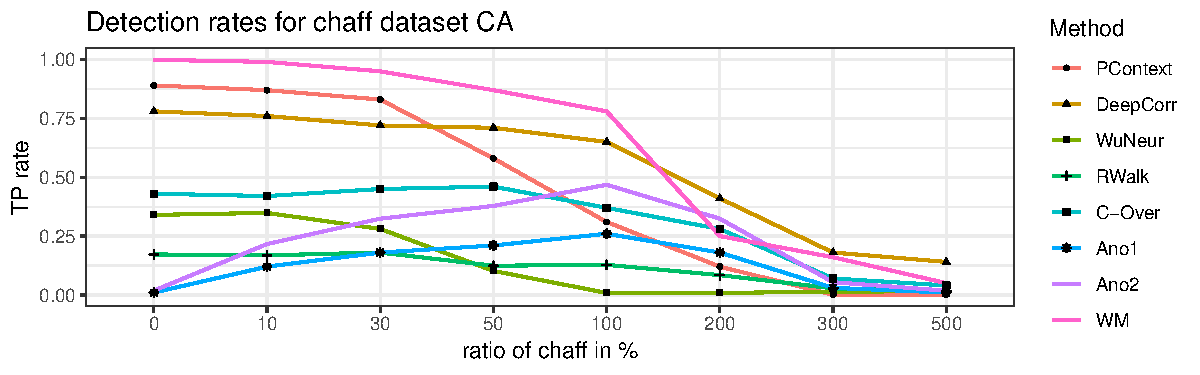
\includegraphics[width=\maxwidth]{figure/Chaffdetection-1} \caption[Detection rates in dependence of $\delta_C$ for different methods on dataset CA with a fixed FP rate of $0.4\%$]{Detection rates in dependence of $\delta_C$ for different methods on dataset CA with a fixed FP rate of $0.4\%$}\label{fig:Chaffdetection}
\end{figure}


\end{knitrout}

As visible, all methods struggle to detect stepping stones once the chaff packets become the majority of the transferred traffic. This is also evident from the AUC-scores given in Table \ref{Tab:AUCchaff}. Several approaches claimed to be resistent to chaff perturbations, however prior evaluations were limited chaff ratios below $100\%$ without obvious reason.

It is surprising that the anomaly detection methods do not perform better at detecting chaff perturbations. Chaff in both approaches was however evaluated with different traffic generation distribution and not compared against a background of traffic following a similar generation distribution, which could explain the disagreement between the results we are finding here.


Overall, these results are in disagreement with the "robustness" claims made for four of the selected approaches, namely PContext, RWalk, Ano1, and Ano2.

\begin{table}
\centering
% latex table generated in R 3.5.3 by xtable 1.8-3 package
% Thu Aug 13 15:10:12 2020
\begin{tabular}{l|r|r|r|r|r|r|r|r}
  \hline
 & PContext & DeepCorr & WuNeur & RWalk & C-Over & Ano1 & Ano2 & WM \\ 
  \hline
AUC & 0.639 & 0.886 & 0.615 & 0.641 & 0.589 & 0.782 & 0.738 & 0.839 \\ 
   \hline
\end{tabular}

\caption{AUC-scores for SSD methods with added chaff at 300\% ratio.}\label{Tab:AUCchaff}
\vspace{-0.7cm}
\end{table}


%\subsection{Combination of delays and chaff}

\subsection{Summary}

Overall, detection rates on dataset BA are mostly in line with the claimed capabilities except for RWalk, although detection rates are slightly lower than stated by most authors. Delay perturbation increases detection difficulty for most methods, except for Ano1, Ano2, and DeepCorr, which contradicts robustness claims for PContext and to some extend WM. Our inserted chaff perturbations however render detection impossible for all methods examined, which contradicts robustness claims for PContext, Ano1, Ano2, and RWalk, even though the claims were based on lower chaff levels. 

As discussed in Section \ref{Sec:Chainl} and \ref{Sec:InfluenceNetwork}, longer chains yield higher detection rates for RTT-based methods while Different network transmission settings seem to have overall little influence on detection rates. 


\section{Related work}\label{Sec:Relatedwork}

\subsection{Testbeds and data}

In 2006, Xin et al. \cite{xin2006testbed} developed a standard test bed for stepping-stone detection, called \textit{SST} that generates interactive SSH and TelNet connection chains with variable host numbers.%, with the goal to enable a reproducible evaluation of stepping stone chain detection algorithms with easy configuration and operation. 
%The tool allows for an arbitrary number of intermediate hosts and generates scripts to mimic interactive SSH and TelNet connections. 
In contrast to our work, the authors give little detail on implemented evasive tactics, and is not available anymore.
%To insert time delays and chaff perturbations, the authors modified the OpenSSH protocol on the intermediary hosts. Delays can be drawn from a uniform distribution while chaff can be drawn from a Poisson or Pareto distribution. 
%To our knowledge, SST has only been used for evaluation by Zhang et al. \cite{zhang2005stepping}, and is not available anymore. %The authors give little details about the implemented evasive tactics.%\textcolor{red}{say something why evasion not sufficiently implemented}

An approach to use publicly available data comes from Houmansadr et al. \cite{nasr2018deepcorr},who simulate stepping stones by adding packet delays and drops retroactively to connections in the CAIDA data \cite{CAIDA2018}.
While this procedure seems sufficient for the evaluation of watermarking methods, it falls short on simulating the effects of an actual connection chain and leaves out chaff perturbations. 
%to evaluate different watermarking methods for SSD. To simulate stepping stone behaviour, packet delays and drops are imposed retroactively on selected connections using Laplace and Bernoulli distributions with different rates. 

We find that when authors evaluate methods on self-generated data, tested evasive behaviours are often lacking analytical discussion and their implementations are too simplistic, leading to increased detection rates. An example of this can be seen in the evaluation of Ano1 \cite{di2011detecting}, where a standard option in netcat is used to generate chaff perturbations for evaluation, or for PContext \cite{yang2015rtt} where simulated chaff is added randomly after the traffic collection.% without consideration of the underlying generation model and its consequences to the detection rates. 
Furthermore, often a relatively low limit on the amount of inserted chaff perturbations is assumed without obvious reason, thus avoiding evaluation at higher ratios. %None of the methods we reviewed evaluate at chaff ratios above $100\%$.

% \textcolor{red}{do we have to back this up with more than just one or two sentences in the discussion? takes up more space...}. 

%\subsection{Surveys}
%Wang et al. \cite{wang2018research} recently conducted an extensive survey of stepping stone intrusion detection. The authors group methods according to the respective methodology 
%\begin{itemize}
%\item content-thumbprint,
%\item time-thumbprint,
%\item packet counting,
%\item random-walk-based,
%\item cross-over packet-based,
%\item watermarking,
%\item network-based,
%\item and software-defined-networking-based, 
%\end{itemize} 
%but do not cover graph-based methods such as \cite{gamarra2018analysis}, %or \cite{apruzzese2017detection}, 
%or anomaly-based methods such as \cite{di2011detecting}.%, which are increasing in popularity recently.
%The authors then proceed to explain the different methods and highlight their benefits and shortcomings as well as open problems. 
%Shullich et al. \cite{shullich2011survey} in 2011 also conducted a survey on stepping stone intrusion detection. The authors perform a similar grouping of methods, but also discuss related work in evasion tactics and test frameworks. The authors furthermore give an outlook on areas for future research, such as hacker motivation, the cardinality problem, or the difficulty of tracing back chains through firewalls.%, the lack of real-world data examples, or detection in covert channels or protocols such as UDP. 
%Neither survey provide an evaluation of detection rates nor a direct comparison of the rates achieved by the corresponding authors. 

%Padhye et al. \cite{padhye2010evading} in 2010 have proposed a packet buffering method to decorrelate packets in the input flow from the output flow. Using this technique and enough chaff packets, the authors generate a constant-rate flow that resembles multimedia streams such as Voice over IP. However, the authors only test their framework against watermark-based SSD methods. 

%Yang et al. \cite{yang2018sniffing} have recently 


%\cite{almulhem2007survey}

%Stepping Stone Detection Techniques: Classification and State-of-the-Art, bad though

%Metrics: A Study on the Performance Metrics forEvaluating Stepping Stone Detection (SSD)
%Stepping Stone Detection: Measuring the SSD Capability
%\subsection{Areas not covered in this work}

%A different direction in SSD that we did not discuss in this work focuses more on the general communication behaviour of selected hosts rather than individual connections. Features include the timely correlation of connecting IP-address on a selected host or unusual paths of simultaneously existing connections within a computer network. 
%Graph-based and behavioural models such as by Apruzzese et al. \cite{apruzzese2017detection} 
%do not examine individual connections but instead 
%focus on the overall temporal activity of hosts in a network. Simulating temporal stepping-stone activity realistically is difficult, which is why we are not able to inlcude these approaches in the evaluation. For the same reason, we did not inlcude \textit{store-and-forward} stepping-stones,  which transfer data in a non-interactive manner and should thus be identified through their temporal behaviour
%Notable examples include Apruzzese et al. \cite{apruzzese2017detection} and Gamarra et al. \cite{gamarra2018analysis}, who both developed graph-based models .
%Simulating temporal stepping-stone activity realistically is difficult, with little empirical data to support specific assumptions. Since our dataset focuses only on individual connections and corresponding evasion, we are not able to include graph-based or behavioural approaches in our evaluation.

%Coskun et al. \cite{coskun2007efficient} identify another form of stepping-stones called \textit{store-and-forward}, which transfer data within files in a non-interactive manner. Though harder to detect than interactive connections, this procedure limits the attackers ability to explore the target, which is why SSD research has been primarily concerned with interactive stepping-stones.


\section{Conclusion}

In this work, we set out to evaluate the state-of-the-art of SSD methods using a comprehensive data generation framework. Our framework simulates realistic stepping-stone behaviour with SSH-tunnels in different  settings and varying amounts of evasive perturbation tactics. 
%The implemented evasive perturbation tactics follow the findings of Padhye et al. \cite{padhye2010evading} to resemble streaming services, and are adjustable in volume. 
We will release a large dataset that highlights multiple aspects in SSD, and is suitable to train ML-based methods. 

Overall, our results show that attackers can reliably evade detection by using the right type and amount of chaff perturbation, which disproves several claims made about the robustness against this evasive tactic. Although to a lesser degree, our implemented delay perturbations still affect detection rates for most methods.% but can be detected by anomaly-based methods.

Currently, it seems that watermarking methods are most suited to reliably detect simple stepping-stones in real-life deployment. The performance of DeepCorr indicates that deep neural networks show the most potential at detecting attacks that use chaff or delay perturbations if they are trained on suitable data. We find that detection and false-positive rates for RTT-based methods are significantly lower than for other methods.%, which makes them less suitable as stand-alone solutions.

\section{Acknowledgments}
%Identification of funding sources and other support, and thanks to individuals and groups that assisted in the research and the preparation of the work should be included in an acknowledgment section, which is placed just before the reference section in your document.

We are grateful to  BT Group PLC who are supporting the PhD research of the first
author in the UK EPSRC CASE scheme, giving invaluable guidance on the needs and possibilities of intelligent security tools and their evaluation. The third author was supported by The Alan Turing Institute under the EPSRC grant EP/N510129/1 and the Office of Naval Research ONR NICOP award N62909-17-1-2065.

%We are grateful for our ongoing collaboration with our industry partners (blinded) on this topic area, who provided both ongoing support and guidance to this work. Discussions with them have helped reinforce the need for a better evaluation and understanding of the possibilities that new tools can provide.

%Full funding sources after currently blinded.

%\bibliographystyle{IEEEtranS}
\bibliographystyle{plain}
\bibliography{NDSSrefs}

\appendix


\section{False positives}\label{Sec:FPana}

Table \ref{Tab:dfFP} depicts the relative contribution\footnote{after adjusting for their weight} at $FP=0.4\%$ of each of the three benign data types to the overall false positive rate. Most methods have more problems with the heterogeneous nature the CAIDA traces, with only PContext and DeepCorr seeing most false positives in the SSH traffic. 

The multimedia traffic is causing most problems for the anomaly-based methods, persumably because it follows a similar distribution as the generated chaff perturbations.
%All methods have little problems identifying the multimedia traffic as benign. 
\begin{table}
\centering
% latex table generated in R 3.5.3 by xtable 1.8-3 package
% Thu Aug 13 15:12:26 2020
\begin{tabular}{l|r|r|r|r|r|r|r|r}
  \hline
 & PContext & DeepCorr & WuNeur & RWalk & C-Over & Ano1 & Ano2 & WM \\ 
  \hline
CAIDA & 0.36 & 0.46 & 0.47 & 0.67 & 0.53 & 0.48 & 0.35 & 0.81 \\ 
  SSH & 0.53 & 0.46 & 0.21 & 0.28 & 0.27 & 0.05 & 0.02 & 0.08 \\ 
  multimedia & 0.11 & 0.08 & 0.32 & 0.04 & 0.20 & 0.47 & 0.63 & 0.11 \\ 
   \hline
\end{tabular}

\caption{Relative contribution in \% of different benign data to the FP rate.}\label{Tab:dfFP}
\end{table}


%\textcolor{red}{I could insert comparison of prediction accuracy on chain length}


\section{Influence of chain length}\label{Sec:Chainl}

In this section, we look at the effect of differing chain lengths on the detection rates. We only focus on RTT-based methods here since the other methods should and do not see a significant effect from varying chain lengths\footnote{For non-RTT-methods, the detection rate error ($2.6\%-6.5\%$) for each length was larger than the detection rate differences ($0.2\%-3.7\%$) across different lengths.}. Since RTT-based methods aim to measure the effect of packets travelling via multiple hosts, it is unsurprising that they perform better at detecting longer chains. 

\begin{knitrout}
\definecolor{shadecolor}{rgb}{0.969, 0.969, 0.969}\color{fgcolor}\begin{figure}
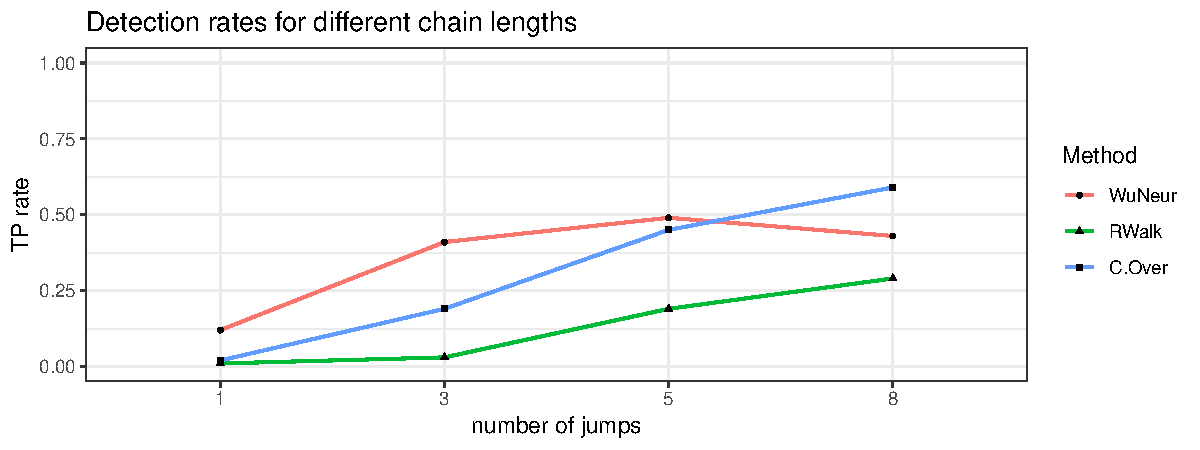
\includegraphics[width=\maxwidth]{figure/Influencechainl-1} \caption[Detection rates in dependence of chain length for different methods on dataset CL with a fixed FP rate of $0.4\%$]{Detection rates in dependence of chain length for different methods on dataset CL with a fixed FP rate of $0.4\%$}\label{fig:Influencechainl}
\end{figure}


\end{knitrout}

%\textcolor{red}{add comparison of results at different positions}

Of the RTT-based methods, only C-Over was able to yield consistent detection rates under transfer delays. 
Interestingly, if the C-Over method is applied to connections between $S_3$ and $S_4$ instead of between $S_4$ and the target, detection rates decrease in the same manner as for other RTT-based methods. This is not surprising as the underlying assumption for robustness for this approach relies on Echo-packets not being delayed.


\section{Influence of network settings}\label{Sec:InfluenceNetwork}

\begin{table}
\centering
\begin{tabular}{l|c|c|c|c|c|c}
& Value & \multicolumn{5}{c}{TP deviation from average}\\ \hline
 & &DeepCorr & WuNeur & RWalk& C-Over & WM \\ \hline
\multirow{2}{*}{RTT} & 5ms& $-0.2\%$ & $+41.3\%$& $-42.3\%$ & $-36\%$ & $+0.03\%$ \\ \cline{2-7}
 & 70ms & $-5.6\%$ & $-5.8\%$& $+35.1\%$ & $+51\%$& $-2.2\%$\\ \hline

\multirow{2}{*}{Packet loss} & $0\%$ & $+1.2\%$& $+1.3\%$ & $+2.1\%$ & $+4.3\%$ & $+0.02\%$\\ \cline{2-7}
 & $7\%$ & $-9.1\%$& $-1.1\%$ & $-3.1\%$ & $-7.3\%$ & $-9.7\%$\\ \hline %\hline

%\footnotesize
%\multirow{2}{*}{\textcolor{grey}{Bandwith}} &\textcolor{grey}{ $0\%$ & $+1.2\%$& $+1.3\%$ & $+2.1\%$ & $+4.3\%$ & $+0.02\%$}\\ \cline{2-7}
%\textcolor{grey}{ & $7\%$ & $-9.1\%$& $-1.1\%$ & $-3.1\%$ & $-7.3\%$ & $-9.7\%$} \normalsize\\ \hline


%\multirow{2}{*}{Bandwidth} & no limit& & & & \\ \cline{2-6}
% & 50 kb/s & & & & \\ \hline s
\end{tabular}
\caption{Influence of network congestion on detection rates at a fixed FP rate of $0.4\%$. The given percentages are describing the change of the detection rate under the given congestion setting when compared to the overall average.}\label{Tab:Congestion}
\end{table}

Finally, we look at the effect of different nework settings. We only show methods that show significant effects and omitted bandwidth from the evaluation as different values do not seem to have any effect on detection rates\footnote{For all methods, the detection rate differences ($0.7\%-6.2\%$) were smaller across bandwidths than the overall detection rate errors ($2.6\%-6.5\%$).}.

As visible in Table \ref{Tab:Congestion}, the three RTT-based methods show different responses to small/large average round-trip-times. While WuNeur, as expected from prior results, performs better in LAN settings, detection rates of the RWalk and C-Over methods are boosted by larger RTTs. All methods profit from lower packet losses.


 

\end{document}
